\documentclass[12pt,letterpaper]{article}

% ---------- Codificación e idioma ----------
\usepackage[utf8]{inputenc}
\usepackage[T1]{fontenc}
\usepackage{mathptmx}          % Times (APA 7)
\usepackage[scaled=.90]{helvet}
\usepackage{courier}
\usepackage{textcomp}

% ---------- Página ----------
\usepackage[margin=0.9in]{geometry}
\usepackage{setspace}
\usepackage{fancyhdr}
\usepackage{titlesec}
\usepackage{enumitem}
\usepackage{booktabs}
\usepackage{longtable}
\usepackage{array}
\usepackage{graphicx}
\usepackage{pdflscape}
\usepackage{afterpage}
\usepackage{caption}
\usepackage[table]{xcolor}
\usepackage[hidelinks]{hyperref}
\usepackage{float}
\usepackage{xurl}
\urlstyle{same}

\IfFileExists{spanish.ldf}{%
  \usepackage[spanish,es-noshorthands,es-nodecimaldot]{babel}%
  \addto\captionsspanish{\renewcommand{\tablename}{Tabla}\renewcommand{\figurename}{Figura}}%
}{%
  \AtBeginDocument{\renewcommand{\tablename}{Tabla}\renewcommand{\figurename}{Figura}}%
}

\setstretch{1.0}
\setlength{\parindent}{0.5in}
\setlength{\parskip}{0pt}
\setlist{nosep, leftmargin=0.35in, itemsep=1pt}

\pagestyle{fancy}
\fancyhf{}
\renewcommand{\headrulewidth}{0pt}
\rhead{\thepage}
\setlength{\headheight}{15pt}
\fancypagestyle{plain}{\fancyhf{}\renewcommand{\headrulewidth}{0pt}\rhead{\thepage}}

\titleformat{\section}[block]{\normalfont\bfseries\centering}{\thesection.}{0.4em}{}
\titleformat{\subsection}[block]{\normalfont\bfseries}{\thesubsection}{0.5em}{}
\titleformat{\subsubsection}[block]{\normalfont\bfseries\itshape}{}{0em}{}
\titlespacing*{\section}{0pt}{10pt}{5pt}
\titlespacing*{\subsection}{0pt}{8pt}{3pt}
\titlespacing*{\subsubsection}{0pt}{6pt}{2pt}

\captionsetup{labelsep=newline, labelfont=bf, textfont=it,
  justification=raggedright, singlelinecheck=false, position=top, skip=3pt}

\definecolor{hdr}{HTML}{EEF0F4}
\newcommand{\code}[1]{{\small\texttt{#1}}}
\newcommand{\tablefont}{\small\setstretch{1.0}}
\newcolumntype{P}[1]{>{\raggedright\arraybackslash}p{#1}}
\newcommand{\adrpart}[1]{\textbf{#1.}~}

\hypersetup{pdftitle={FraudLens: detección de fraude en pagos digitales en tiempo real},
  pdfauthor={Vélez, Samper, Salazar, Yanes}}

\begin{document}

% ======================= PORTADA =======================
\thispagestyle{plain}
\setstretch{1.5}
\vspace*{1.4in}
\begin{center}
{\bfseries FraudLens: detección de fraude en pagos digitales en tiempo real\\[2pt]
Entregable 1: diagnóstico, requisitos y arquitectura\\[2pt]
Dominio: fintech colombiana (billetera digital y pagos inmediatos)}

\vspace{0.45in}
Andrés Felipe Vélez Álvarez (1021923619; afveleza@eafit.edu.co)\\
Samuel Samper Cardona (1040180930; ssamperc@eafit.edu.co)\\
Sebastián Salazar Henao (1022003377; salazarh3@eafit.edu.co)\\
Hellen Yanes Doria (1026137704; hyanesd@eafit.edu.co)

\vspace{0.4in}
Universidad EAFIT\\
ST1630 Sistemas Intensivos en Datos\\
Profesor: Andrés Sacre Alzate\\
11 de octubre de 2026

\vspace{0.3in}
{\small\setstretch{1.0}Repositorio: \url{https://github.com/AndresVelez31/st1630-252} (rama \texttt{fraudlens-entregable1}, carpeta \texttt{proyecto-final/fraudlens/})}
\end{center}
\clearpage
\setstretch{1.0}

\begin{center}
{\bfseries FraudLens: detección de fraude en pagos digitales en tiempo real}
\end{center}

% ======================= SECCIÓN 1 =======================
\section{Definición del problema}

\subsection*{1.1 Contexto y problema de negocio}

Los pagos digitales en Colombia crecen a un ritmo que los controles diarios ya no alcanzan. Bre-B, el sistema de pagos inmediatos del Banco de la República, procesó más de 1.700 millones de transacciones por más de \$262 billones en su primer año y suma más de 36 millones de usuarios (Banco de la República, 2026); el 62~\% de esas operaciones es menor a \$50.000. Nequi, la billetera más grande del país, reporta más de 50 millones de transacciones diarias con 27 millones de usuarios (ABC Economía, 2025). El fraude crece con ellos: Asobancaria registró más de 218.000 reclamos por fraude en canales financieros solo en el primer semestre de 2025, y el 36,6~\% de los colombianos dice haber sido víctima directa de un fraude en el último año (Suárez, 2026).

FraudLens es una billetera digital colombiana (empresa ficticia, proyecto académico) conectada a Bre-B que procesa pagos con QR, transferencias inmediatas y pagos a comercios. Hoy su equipo de riesgo detecta el fraude con reportes que se calculan al cierre del día sobre la base de datos operacional. Cuando un analista ve un patrón sospechoso, como una ráfaga de transferencias pequeñas hacia un comercio recién creado o un pago desde un dispositivo nunca visto en otra ciudad, el dinero ya salió: una transferencia inmediata se liquida en segundos y no se puede reversar.

\textbf{El problema:} los analistas de riesgo de FraudLens necesitan detectar patrones de fraude en menos de 2 minutos desde que ocurre la transacción sospechosa y, además, analizar el histórico completo para ajustar las reglas con evidencia, sin afectar el rendimiento de la app de pagos.

\subsection*{1.2 Usuarios del sistema y decisiones que toman}

\begin{table}[H]
\caption{Usuarios del sistema y decisiones que toman con los datos}
\tablefont
\begin{tabular}{@{}P{1.4in}P{3.4in}P{1.55in}@{}}
\toprule
\textbf{Usuario} & \textbf{Decisión que toma con los datos} & \textbf{Urgencia}\\
\midrule
Analista de fraude & Bloquear una cuenta, pedir verificación adicional o descartar una alerta. & Minutos desde el evento\\
Jefe de riesgo & Ajustar umbrales de las reglas (montos, ventanas) según la tasa de fraude por comercio, ciudad y franja horaria. & Semanal\\
Equipo de comercios & Suspender o poner en revisión a comercios con montos sospechosos recurrentes. & Diaria\\
Auditoría y cumplimiento & Verificar de dónde salió una cifra y reconstruir el estado de los datos en una fecha pasada. & Bajo demanda\\
\bottomrule
\end{tabular}
\end{table}

\subsection*{1.3 Preguntas que el sistema debe responder}

\textbf{Operacionales (tiempo real, alerta en menos de 2 minutos):}
\begin{itemize}
  \item P1. ¿Qué clientes superan 5 transacciones o \$2.000.000 acumulados en una ventana de 5 minutos?
  \item P2. ¿Qué transacciones vienen de un dispositivo nunca visto para ese cliente y con un monto mayor a 3 veces su promedio de los últimos 30 días?
  \item P3. ¿Qué pagos involucran un comercio o un dispositivo de la lista de riesgo vigente?
\end{itemize}
\textbf{Analíticas (capa Gold, datos con máximo 15 minutos de antigüedad):}
\begin{itemize}
  \item P4. ¿Cuál es la tasa de fraude (\% de transacciones y \% del monto) por comercio, ciudad y franja horaria, semana a semana?
  \item P5. ¿Cuál es la latencia promedio y en el percentil 95 entre la transacción y su alerta, y cuántas alertas dispara cada regla?
  \item P6. ¿Cuáles son los 10 comercios con mayor monto sospechoso en los últimos 7 días?
\end{itemize}

\subsection*{1.4 Por qué se necesita una arquitectura de datos distribuida}

El volumen por sí solo no descarta una base relacional grande; lo que la descarta es la combinación de cinco condiciones (el dimensionamiento completo está en el Anexo A):
\begin{itemize}
  \item \textbf{Volumen y velocidad.} Se diseña para 1.000 eventos/s en promedio, por encima del promedio de Nequi ($\approx$580 transacciones/s) para absorber el crecimiento de Bre-B, con picos de 5.000 eventos/s en quincena, Día sin IVA y diciembre. Son unos 86 millones de eventos y 86 GB de JSON al día.
  \item \textbf{Estado por cliente en tiempo real.} P1 y P2 exigen ventanas de 5 minutos y promedios de 30 días por cliente, recalculados de forma continua. Hacerlo con consultas SQL sobre la tabla transaccional competiría con los pagos en curso.
  \item \textbf{Cargas mezcladas.} La app necesita escrituras rápidas y consistentes (OLTP) y los analistas, agregaciones sobre meses de histórico (OLAP). Separarlas evita que una consulta pesada degrade los pagos.
  \item \textbf{Variedad.} Llegan eventos JSON continuos, tablas relacionales de clientes y comercios y archivos CSV de listas de riesgo, cada uno con su formato, frecuencia y calidad.
  \item \textbf{Reprocesamiento y auditoría.} Cuando cambia una regla hay que recalcular sobre el histórico y poder reconstruir una fecha pasada, lo que exige almacenamiento inmutable y versionado, no tablas que se sobrescriben (Kleppmann, 2017).
\end{itemize}

% ======================= SECCIÓN 2 =======================
\section{Requisitos funcionales y no funcionales}

\subsection*{2.1 Requisitos funcionales}

Cada requisito se ubica en una capa del diagrama (Sección 3), es verificable en la demo y, cuando aplica, indica qué pregunta de la Sección 1.3 responde.

\begin{footnotesize}\setstretch{1.0}
\setlength{\LTpre}{4pt}\setlength{\LTleft}{0pt}\setlength{\LTpost}{2pt}
\setlength{\tabcolsep}{4pt}
\begin{longtable}{@{}P{0.45in}P{2.85in}P{0.95in}P{2.05in}@{}}
\caption{Requisitos funcionales}\\
\toprule
\textbf{ID} & \textbf{Requisito funcional} & \textbf{Capa} & \textbf{Verificación}\\
\midrule
\endfirsthead
\toprule
\textbf{ID} & \textbf{Requisito funcional} & \textbf{Capa} & \textbf{Verificación}\\
\midrule
\endhead
\midrule
\multicolumn{4}{r}{\emph{Continúa en la página siguiente}}\\
\endfoot
\bottomrule
\endlastfoot
RF-01 & El sistema debe ingerir en tiempo real los eventos de transacción (pagos QR, transferencias inmediatas y pagos a comercios) en el topic \code{transacciones} de Kafka, con clave \code{id\_cliente} y latencia menor a 5 s desde su generación. & Fuente $\rightarrow$ Ingestión & El productor sella cada evento; se mide el tiempo hasta que está en el topic.\\[1pt]
RF-02 & El sistema debe cargar cada día los catálogos de clientes y comercios desde PostgreSQL 16 hacia Bronze. & Ingestión batch & El DAG \code{catalogos\_diario} registra la carga y Bronze tiene la versión del día.\\[1pt]
RF-03 & El sistema debe importar a Bronze cada versión nueva de los CSV de listas de riesgo (comercios y dispositivos) apenas se publique en \code{s3://\ldots/landing/}. & Ingestión batch & Al subir un CSV, el sensor dispara la carga y aparece una versión nueva. Soporta P3.\\[1pt]
RF-04 & El sistema debe persistir los eventos crudos sin modificarlos en Bronze (Delta Lake en S3) con su topic, partición, offset y \code{ingest\_ts}. & Bronze & Los \code{id\_transaccion} distintos en Bronze coinciden con los eventos únicos producidos.\\[1pt]
RF-05 & El sistema debe validar, deduplicar por \code{id\_transaccion} y estandarizar los eventos hacia Silver; el JSON ilegible va al topic \code{transacciones\_dlq} y lo que incumple reglas de calidad, a una tabla de cuarentena con el motivo. & Procesamiento $\rightarrow$ Silver & Se inyectan duplicados, JSON roto y montos negativos: Silver solo tiene registros únicos y válidos y cada rechazo está en la DLQ o en cuarentena.\\[1pt]
RF-06 & El sistema debe contar transacciones y sumar montos por cliente en ventanas deslizantes de 5 min que avanzan cada minuto, y alertar al superar 5 transacciones o \$2.000.000. & Procesamiento (streaming) & Una ráfaga de prueba dispara la alerta. Responde P1.\\[1pt]
RF-07 & El sistema debe alertar cuando una transacción venga de un dispositivo nunca visto para el cliente y su monto supere 3 veces su promedio de 30 días. & Procesamiento (streaming) & Caso con dispositivo nuevo y monto alto. Responde P2.\\[1pt]
RF-08 & El sistema debe alertar cuando un pago involucre un comercio o un dispositivo de la versión vigente de la lista de riesgo. & Procesamiento (join) & Pagos a un comercio listado disparan alerta. Responde P3.\\[1pt]
RF-09 & El sistema debe registrar cada alerta (regla, transacción, cliente, comercio, hora del evento y de la alerta) en MongoDB y en Silver sin duplicarla, y notificar por Amazon SNS solo las alertas nuevas. & Almacenamiento $\rightarrow$ Consumo & Tras reiniciar el job a mitad de un lote, el número de alertas y de correos no cambia.\\[1pt]
RF-10 & El sistema debe construir en Gold un esquema en estrella: hechos de transacciones y de alertas; dimensiones de cliente (SCD tipo 2), comercio, dispositivo, tiempo y regla. & Gold & Una consulta con joins entre hechos y dimensiones devuelve resultados correctos.\\[1pt]
RF-11 & El sistema debe calcular en Gold la tasa de fraude por comercio, ciudad y franja horaria, con corte semanal. & Batch $\rightarrow$ Gold & Consulta en Athena. Responde P4.\\[1pt]
RF-12 & El sistema debe calcular en Gold la latencia promedio y P95 entre transacción y alerta, y las alertas por regla. & Batch $\rightarrow$ Gold & Consulta en Athena. Responde P5.\\[1pt]
RF-13 & El sistema debe listar los 10 comercios con mayor monto sospechoso de los últimos 7 días. & Gold $\rightarrow$ Consumo & Consulta en Athena. Responde P6.\\[1pt]
RF-14 & El sistema debe permitir consultar Gold con SQL en Amazon Athena (tablas registradas en AWS Glue) y mostrar dashboards de fraude en Metabase, sin tocar la base operacional. & Consumo & Un analista ejecuta P4--P6 en Athena y las ve en Metabase.\\[1pt]
RF-15 & El sistema debe orquestar con Airflow tres DAG: \code{catalogos\_diario} (diario o al llegar un CSV) \code{fraude\_pipeline} (Silver $\rightarrow$ Gold, calidad y registro en Glue, cada 10 min) y \code{sesion\_aws} (crea la infraestructura y restaura el respaldo al iniciar cada sesión de AWS). Un fallo debe detener los pasos dependientes y una tarea debe verificar que el streaming esté vivo. & Orquestación & Un fallo forzado detiene los pasos siguientes; si se detiene el streaming, Airflow lo reporta.\\[1pt]
RF-16 & El sistema debe reprocesar un rango de fechas con una versión nueva de las reglas (\code{rule\_version}) escribiendo el resultado en Gold, sin modificar Bronze ni Silver. & Batch $\rightarrow$ Gold & Se reprocesa un día y se comparan las dos versiones.\\[1pt]
RF-17 & El sistema debe exponer las alertas en una API REST (FastAPI) consultable por cliente, regla y rango de tiempo. & Consumo & \code{GET /alertas} devuelve la alerta de la ráfaga de prueba. Soporta P1--P3.\\
\end{longtable}
\end{footnotesize}

\subsection*{2.2 Requisitos no funcionales}

Los valores parten del dimensionamiento del Anexo A y de la meta de detección en menos de 2 minutos. La terminología de CAP y de garantías de entrega sigue a Kleppmann (2017); el tratamiento de datos personales, a la Ley 1581 de 2012.

\begin{footnotesize}\setstretch{1.0}
\setlength{\LTpre}{4pt}\setlength{\LTleft}{0pt}\setlength{\LTpost}{2pt}
\setlength{\tabcolsep}{4pt}
\begin{longtable}{@{}P{0.8in}P{3.95in}P{1.7in}@{}}
\caption{Requisitos no funcionales}\\
\toprule
\textbf{ID / concepto} & \textbf{Requisito no funcional (valor concreto)} & \textbf{Cómo se verifica}\\
\midrule
\endfirsthead
\toprule
\textbf{ID / concepto} & \textbf{Requisito no funcional (valor concreto)} & \textbf{Cómo se verifica}\\
\midrule
\endhead
\midrule
\multicolumn{3}{r}{\emph{Continúa en la página siguiente}}\\
\endfoot
\bottomrule
\endlastfoot
RNF-01 Escalabilidad & Capacidad de diseño: 5.000 eventos/s sostenidos 30 min sin que el lag del consumidor crezca. El topic tiene 12 particiones (hasta 12 tareas de Spark en paralelo, $\approx$420 eventos/s por partición en el pico). Crecer a 10.000 eventos/s debe requerir solo más brokers y ejecutores, o mover el cómputo a EMR, sin cambiar código ni el almacenamiento en S3. Las particiones se fijan desde el inicio porque aumentarlas cambia la partición de cada \code{id\_cliente} y rompe el orden por cliente. & Prueba de carga escalonada en el portátil de la demo; se reportan el máximo sostenido y el lag.\\[1pt]
RNF-02 Disponibilidad (CAP) & La posición CAP se define por componente. \textbf{Kafka: CP}, con 3 brokers, replicación 3, \code{acks=all} y \code{min.insync.replicas=2}: con menos de 2 réplicas sincronizadas rechaza escrituras antes que aceptar pagos que puedan perderse. \textbf{S3: CP}, con consistencia de lectura tras escritura (Lab 1a). \textbf{MongoDB: CP en escritura y disponibilidad priorizada en lectura}: replica set de 3 nodos, escrituras con \code{w=majority} y lecturas de los analistas con \code{secondaryPreferred}, que siguen respondiendo si cae el primario (ADR-04). Metas: 99,5~\% en ingestión y 99~\% en consulta de alertas. & Se detiene un broker y luego el primario de MongoDB: la ingestión y la consulta siguen; con dos brokers detenidos, el productor recibe error en vez de perder datos.\\[1pt]
RNF-03 Consistencia (garantía de entrega) & Ingestión at-least-once (\code{acks=all}, reintentos, productor idempotente). De Kafka a Silver y Gold el efecto es exactly-once: checkpoint de Spark junto a los datos en S3 y escrituras idempotentes con \code{MERGE} por \code{id\_transaccion}. Las alertas se escriben con \emph{upsert} sobre un \code{\_id} determinista (hash de cliente, regla y ventana, o de la transacción), y SNS solo notifica cuando el \emph{upsert} insertó un documento nuevo. Bronze admite duplicados; Silver, Gold, MongoDB y los correos, cero. & Se mata el job a mitad de un micro-batch: los conteos de Silver, MongoDB y correos no cambian.\\[1pt]
RNF-04 Latencia & Evento $\rightarrow$ alerta: 30 s en P95 y 60 s como máximo (trigger de 5 s; R1 emite en modo \code{update} sin esperar el cierre de la ventana). Evento $\rightarrow$ Gold: 15 min (\code{fraude\_pipeline} cada 10 min). Consultas de Athena sobre 30 días: menos de 10 s, gracias a la partición por fecha y a \code{OPTIMIZE ZORDER} (Lab 1b). & Hora del evento contra hora de la alerta (RF-12) y tiempo de ejecución de Athena.\\[1pt]
RNF-05 Tolerancia a fallos & Si cae un broker, Kafka sigue sin perder escrituras confirmadas. Si cae el job de Spark, el contenedor se reinicia y retoma desde su checkpoint en menos de 5 min (RPO = 0 para eventos en Kafka, retenidos 7 días). Si termina la sesión de AWS, el sandbox borra el bucket: \code{sesion\_aws} lo recrea y restaura el último respaldo en menos de 15 min, y lo que falte se reprocesa desde Kafka sin duplicar gracias al \code{MERGE}. Airflow reintenta cada tarea 3 veces con espera exponencial y luego detiene los dependientes y notifica. & Se apaga un broker, el primario de MongoDB y el job de streaming durante la demo y se cronometra la recuperación; se ensaya \code{sesion\_aws} desde cero.\\[1pt]
RNF-06 Trazabilidad & Silver y Gold conservan \code{source\_system}, \code{kafka\_partition}, \code{kafka\_offset}, \code{ingest\_ts}, \code{batch\_id} y \code{rule\_version}. Delta conserva 90 días de historial para time travel (en el sandbox, mientras el respaldo lo preserve). Toda cifra de Gold se rastrea hasta sus eventos de Bronze. & Se sigue una cifra de Gold hasta Bronze y se consulta \code{VERSION AS OF}.\\[1pt]
RNF-07 Seguridad y privacidad & Documento, teléfono y correo se reemplazan desde Silver por un HMAC-SHA-256 con clave fuera del repositorio (un hash simple se revierte por fuerza bruta). S3 cifra en reposo (SSE-S3) y bloquea el acceso público; las API de AWS usan TLS. Las credenciales temporales del sandbox van en un \code{.env} excluido de Git. Solo auditoría lee Bronze con datos originales (Ley 1581 de 2012). & Las consultas de Athena y Metabase no devuelven datos personales en claro.\\[1pt]
RNF-08 Calidad de datos & Los registros inválidos no detienen el pipeline: van a la DLQ o a cuarentena con su motivo; si la tasa de rechazo de una ejecución supera 1~\%, \code{quality\_checks} falla y notifica. & Se inyectan registros inválidos y se revisa la tasa.\\[1pt]
RNF-09 Costo & El proyecto completo (desarrollo, pruebas y demo) debe costar menos de USD 50, el crédito de AWS Academy. Solo se usan servicios que cobran por uso (S3, Athena, Glue, SNS); no se crean EC2, volúmenes EBS, IP elásticas, RDS, snapshots, secretos ni métricas de CloudWatch, que cobran aunque no haya instancias encendidas (Anexo B). & Revisión del presupuesto del sandbox al iniciar cada sesión (AWS Budgets se actualiza cada 8 a 12 h).\\
\end{longtable}
\end{footnotesize}

% ======================= SECCIÓN 3 =======================
\section{Diagrama de arquitectura de datos por capas}

La Figura 1 (página siguiente) muestra las cinco capas del pipeline como franjas horizontales, de la fuente al consumo, y usa la notación oficial de AWS (AWS Architecture Icons de draw.io) para el despliegue. A la izquierda, el grupo \emph{equipo local} reúne lo que corre en contenedores con Docker Compose: productor, Kafka, Spark, Airflow, PostgreSQL, MongoDB, Metabase y FastAPI, cada uno con su perfil (\code{streaming}, \code{batch} o \code{consumo}). A la derecha, los grupos \emph{AWS Cloud} y \emph{Region} contienen los servicios administrados del sandbox: el bucket de S3 con los prefijos Bronze, Silver y Gold, Glue Data Catalog, Athena, SNS y la pila de CloudFormation que los crea en cada sesión. Cada componente nombra la herramienta concreta. Los archivos fuente están en el repositorio (\path{arquitectura.drawio}, \path{arquitectura.png} y \path{arquitectura.svg}) y el diagrama se puede editar en línea desde el enlace de la nota.

\afterpage{%
\clearpage
\newgeometry{margin=0.45in}
\begin{landscape}
\thispagestyle{plain}
\setstretch{1.0}
\begin{center}
\captionof{figure}{Arquitectura de datos por capas de FraudLens (cómputo local y servicios del sandbox de AWS Academy)}
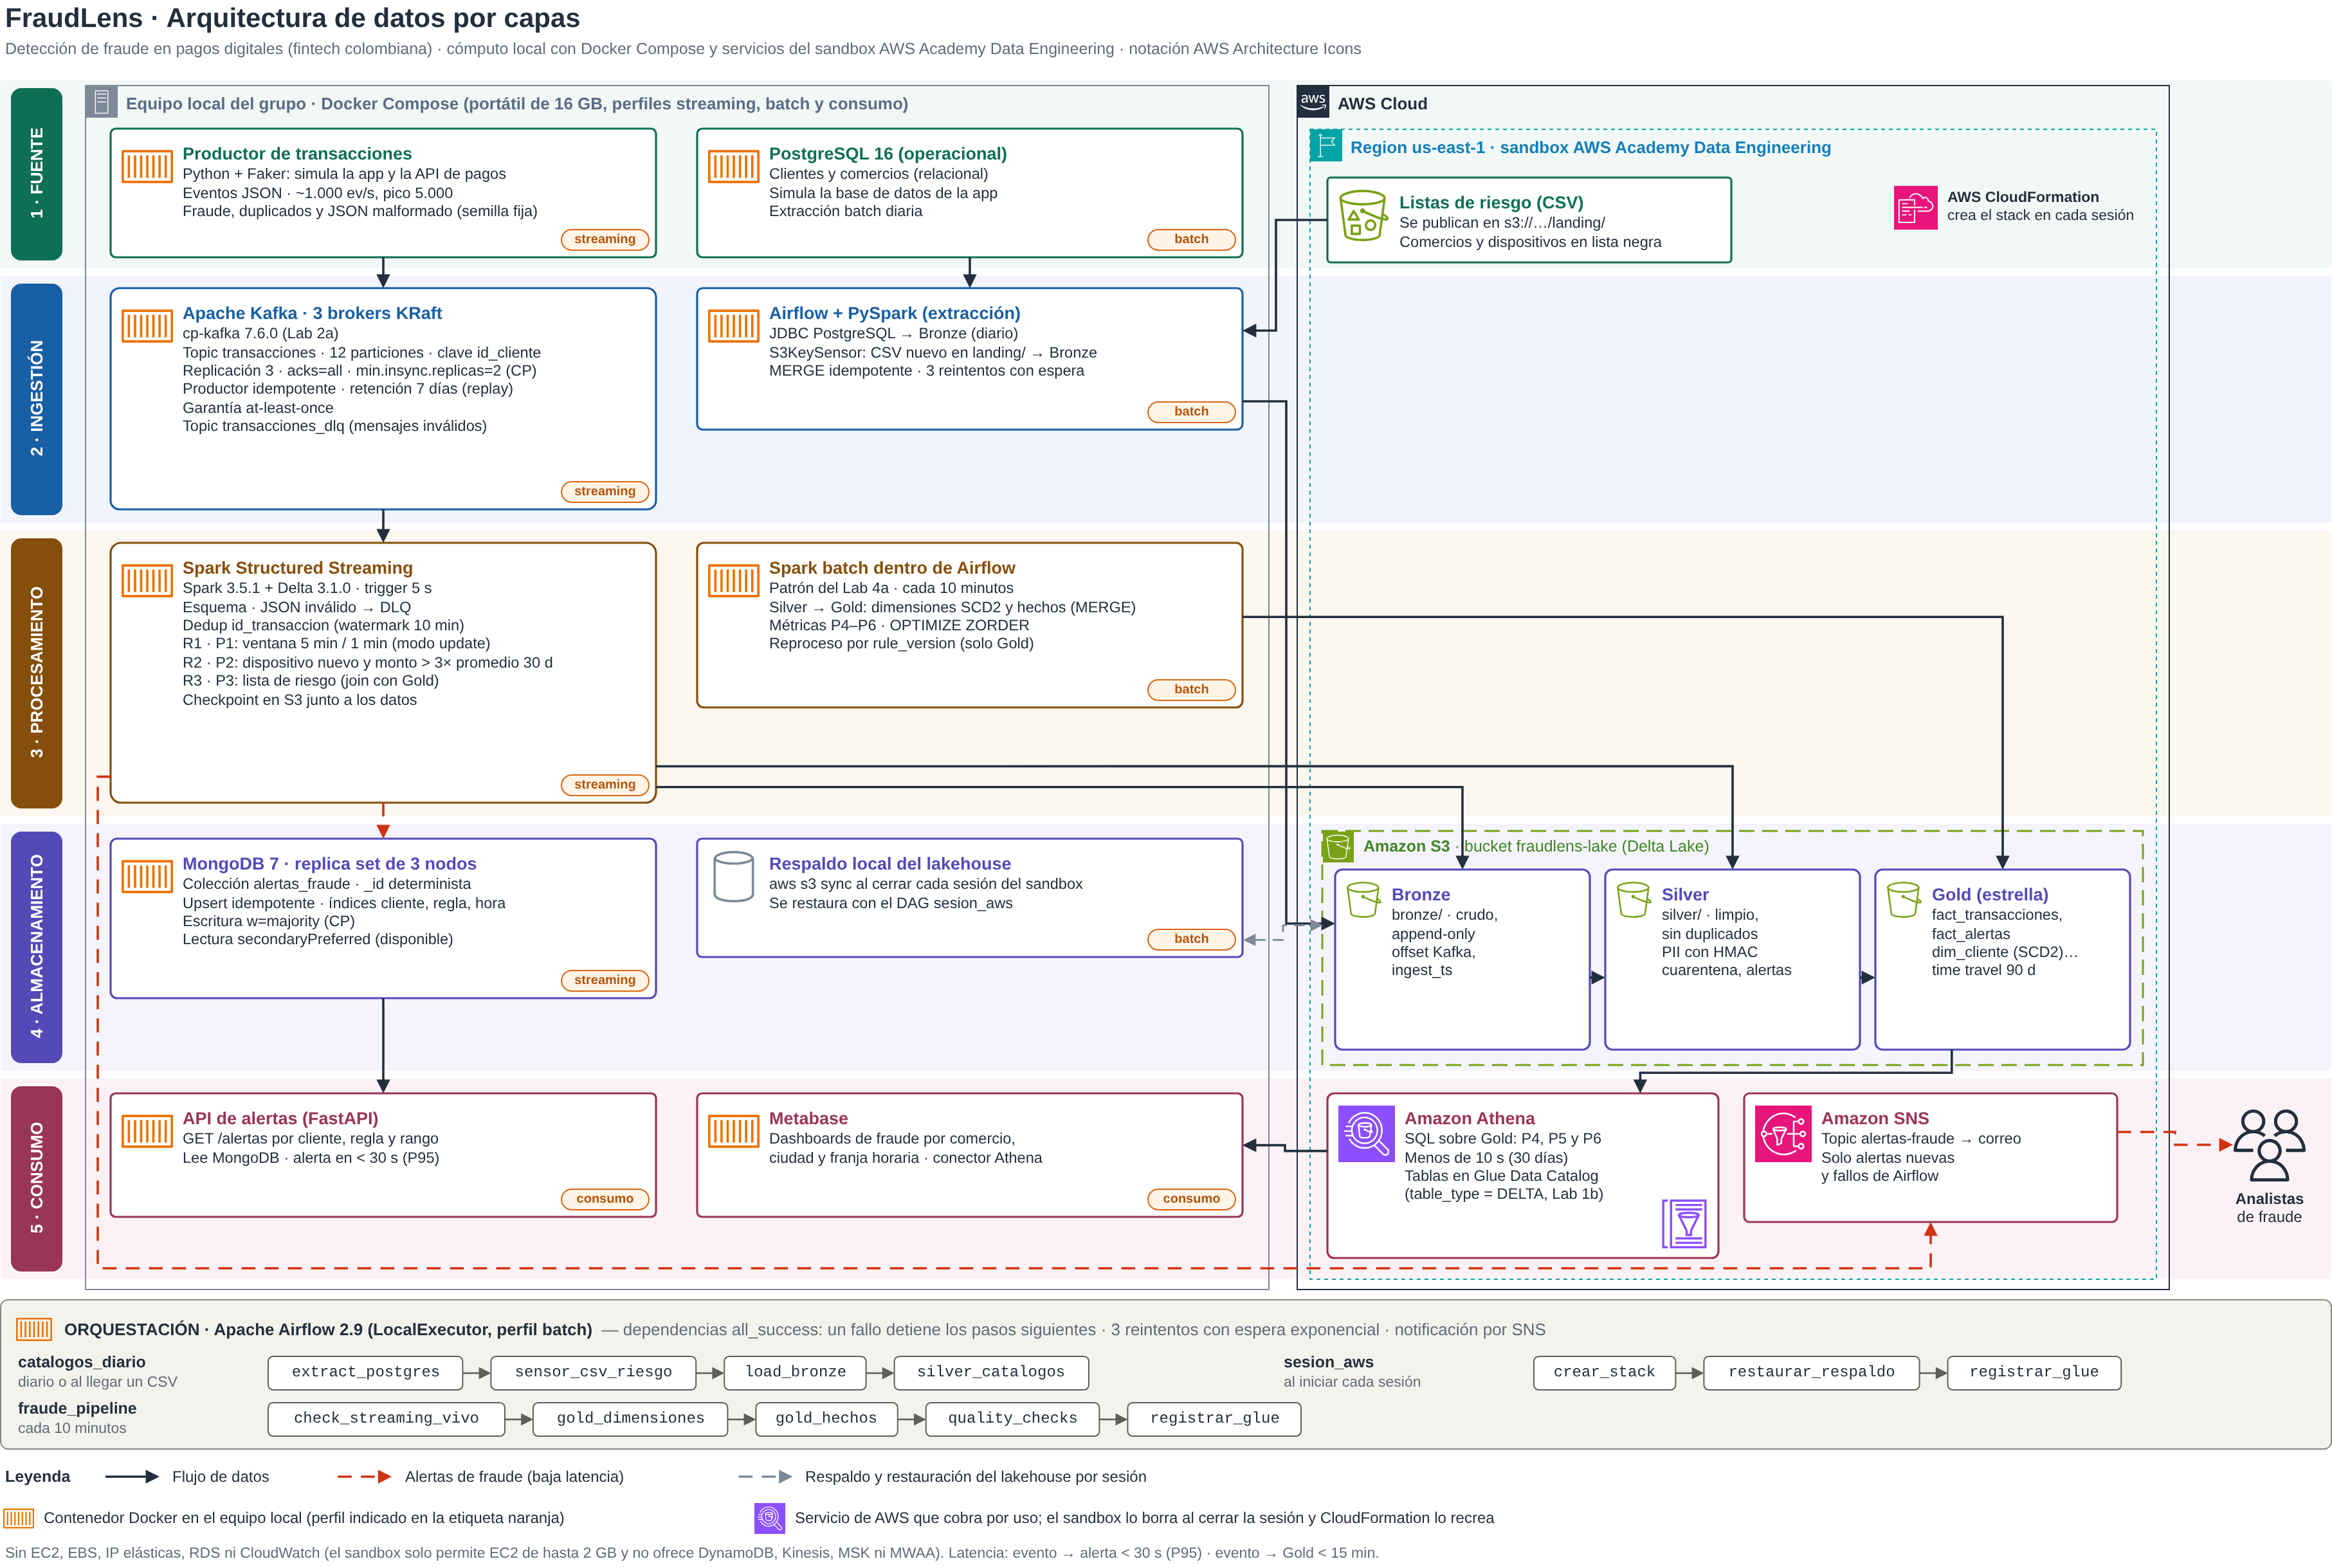
\includegraphics[width=\linewidth,height=6.75in,keepaspectratio]{img/arquitectura.png}

\vspace{2pt}
\raggedright\small
\emph{Nota.} Enlace editable en draw.io: \href{https://app.diagrams.net/\#R7V3Jdts4Fv0aL6PDWdRS1pBKl524rFRXd290IBKWGFMEQ5COXYv\%2B9sZEigNk0TYHy81UTkqkOEDAfcDFGy\%2F02f7xzvPhhabsEI4v9PmFpoEwHLke2EZgj0cBjMmpC31xoc\%2FESXKx5\%2FJL7yKQuD4M8CcQ\%2FaTXaUoA9pB\%2FOY1\%2BJl4MnTiJAPliSa\%2B9Itdmz9s\%2Ffo5AuLtGLvTJBe4jv0\%2B1DYU\%2Fy30SZzTd4me2Ufpq5XBi5f0tXqmmZxPPhVic46dihPzYC4snHRQEpIGFcyCK0K\%2FiZXfIdwsnQrCFlRMrB\%2FjVs395brwr\%2FzD6xW\%2FQ2\%2B7i8g\%2FcAOd\%2BG6EkEC\%2B80PQl\%2B8O\%2F3oP0YeJJeAdc9Ct3ivVshFCc9vEM\%2Bn5uyPh9yyPfZg2PYBDXuSH2YgofetMD8BOYttryye2XG\%2FJhSz\%2FkBl\%2B5mGkXl2PyoQQQl8LQBTGiF4UoouMDQoDTh5FGZM8TPz5\%2BSns8ho\%2F0\%2FC7e\%2B\%2BSESj4SXPsz5JPn6PMABeS6SxxH6B6WTgLf2wbk0Id39AkPMIo9MpJTcXrvuS59yeWvHWnrKgQOfeMvAlz6DhTEAn2aKo7Tx5ORI\%2F8tabfx60RjFXG8BHvPpwD\%2FDfoPkL4z\%2B120DfDx6IioeQmCaA\%2Fj6Ilckt4gkCRkx\%2BZHv3Iw1BQBnl0OgumFQEB\%2Fmz34MPrkgwCAHAw42cjxMIdkmB3vYqZfXOpBOtZs9qAfYMBlgo286229mEgSg4pm33kBuXfHhNVH\%2B40HAgKWSR5HDn\%2FuPkxiRA59RIaPCzf5d46ce0ixNEP7EGHIeoZAB0YPnuPxN7LpB4PA3aBHisu\%2FVvRfB7hwT6\%2Bdg5jicxFsvQDCyAu2\%2BbcHKAb5nybujpydwDZ95RfSGPz\%2BQKtqI7MKW3NpXY6n\%2FcI2nQ\%2FzuDWluFXejtsNGXpFMomVhotNy9BNOyM3VHSWVpf20jw2XrkhbqKvjEJfjZVqX9mqVu0r1bDe3lk7N6r2lZqXiOWfi6\%2FfF890H\%2B0GEDnpzKkUO2iHIu9vgjTgy3taWVoL0zrW0yUsi8WziGW1JAV6y9hOsZSOVxXbhgTZqm40A2317dA2l5e9QDvrutPYnmiNYLvaWVoe21\%2B\%2Bfl6svn\%2Bh0\%2F1E\%2F9oaxlXbXE7NM8a4jHhIQW43NH9rbwX5bDleLHsBuaHVncCzXn4jyKudpedBfnP7bbZYTa\%2B\%2FkHn8W2sYt01jqVyeMcYNrd5Enm1L34px\%2Fa0YN5fGctYLxi3D7ngir3aWUdh8Xl1PZ4uvbYPc1I0ped\%2F5gtwyjW4ncuPtE7m2tHoBuW1YdUFuNsPEq51l5kE\%2B\%2B\%2FZ19ed1e\%2BieTHTzrKm4bWr10G00wMW3a6GaKA3Z4mfihXnNBVdIbKOEnc1GU6LKuNDsEEUxpaNTNfb8VLVCd9PKZ9JhM9o7MKJKXswwEEHSs1SDMWPaxpipVp64ugQne8R0KyW4hMgLYvbDzUvyl7x1plyYc\%2FoMcjSimCucKB\%2BPiyfU6hF9RvFE\%2BXhcPKGWH6\%2BW3q\%2BWG5g7UTkqPF4pvV\%2FJNZD81S9REvteQNCeKo\%2BpZGwj4HrwAPjqfHNKF6NLRMOhwkfeFYm3sJGA0eIB8gFR2DW\%2BD0LsbTI9TQSdJMLeA7yFmD\%2BcnsU7ENLP\%2B8ctVbuPwC9sjKiuOWTNpyoq6bdrFKzDCO49XFVHEbEez\%2B3JxJbrrsp6qRiFVeUVJl1CEHnFjua6IlFITa2ZTacZF\%2BDdYd5vcZpIF7N0x15dAyeaZJqY6FYT04Tjo8StTBNcsTg7fDdI6CChXELJRw6aNWCmkoqQHiwRrQlp9orOhFRVyoq1qphaY7s1MY3g1qM2hpKc3orTSoI\%2FQYDjTwXl6MvMDIOYD2J\%2BEHMBOIl8K8rUmFqtyrdqjBeX07x8q63Lt16Ub1WpKhEsUyLg9qQBuu7cBWvv9GZUKpNSuZTJplQ\%2BqzJauIxJjeQNquQNquwNVblXK2\%2BoziZCGqvnZLNK\%2BW5VcrdaupvJNL6HdE\%2FCJUUq4EeN7MW96WKsmuNLmbDcsT\%2FllSoVkyuwgf4Nwl7MZG2\%2BQXGM9iflyIF0PihZc\%2FOWVok9FeCQ\%2F6w775G2Qz4zRBCjJHIgnxfInIJlMwRb\%2Fu9QtAe83c2oN\%2ByiVVaVbJdTK1Ve\%2FvSGxC8\%2B7VmSY8XL7NdLPUbEjVF6xiFbYep8wIz\%2FMXDuU08EsiID5iKAD2b9d2e5V2WW\%2B34cTkytjBKJPcOSwaQBn5MwQu5LNIZFhZdxfBDzGqvqelu0QadOXurIamrpU06ufIYm6dLsxrf2aZ2l7\%2FVz9RGSVp7C52P6e45I0rubvcucUD02o2dkct2UHjqFRwoXdVxLrWk0BZZnJ\%2BocZKyfCfVMZH35iVPiqaqPzPCR82c6vtODfGXXp3P2DXlZ4sTMOZApOuMIBBg4DhltiOvN\%2B\%2BkZQnmD041TR3a5cQLF1cY9xTu28bvQLqkbDKDaWnqHgr194tM1hf0DwlDoXNnh9OZL\%2BmuED1y5xQxRzFXtH6tvX\%2FO7yf\%2BqI4VKvAIfyI\%2FGQt\%2FrOVRvbPKvyg9bCq87eqWbhD4RCpc9\%2B\%2Bnw\%2FD3wGZVwEdcxY0iWDtbYO\%2B8Hd7\%2FLepp3Y9dumVx8ZYuk2Ml8pxfMtdbXPqMkeGqVIFmWRAVhNCV5YFuRvZyWv\%2BY6aCqnFkJjYcoWwrltWdmGOXf\%2B0jB1ZtzPz6KKZGNdmYGPMqI2x9EwS\%2ButXbXkWZKNptqAIincfjz\%2BYppWn\%2FxlO7CXM2IvpmX0x1623XEXhONtBFd\%2FXKUGWrKyohBGgLIXavid9ExgZj5FNcSZRXgPI\%2BEjT5oaQb\%2Fa0kOrVgWOswHMPl2I6WAHBwZUYTmPhMwVogRS87TrgcgDA\%2BcQ65Cq9Mg5tlLGIUZqYBu1RnCiWL2xDQc\%2FfER1iVHqUYknlq5K\%2BIbVTJe\%2BB74xnpLJ3vp4fGOTOKTn1r\%2B8eLdGmx\%2FkKbgp1JR3b6bZGfGgoOmKeVx5OAbZChx5EG\%2FFxn62\%2Bmf\%2FtGPFVB\%2FJhqoiglQJj3V205L\%2BXWgXtnIxJb9s6YPAZRvbZbWBsxxfeWK0AYcM2w\%2FsFHusT7uCRu3BbTQwivSGirrZmFQEQTMllMJqQBLuwd096H5NKoXYtK7C13St5hZ4rDXUqcMu\%2BIx1\%2BJqhdrYYcbQ0vRwJCavM91Myt\%2B3onP87l\%2FyDOptGIW0oTCI6Yf9\%2BC8is2e\%2Fa5ISfxPykjEfWSOHLJkEo\%2BaAB6UaYzNmeUzVNHH6lKoARe9XvHB88QDYya4fvxqsvuIVMa5\%2FfKRfCt4BzT7EA2BBnZ\%2FdeMPIC\%2FBQ4o4g\%2FALOlhfOAG\%2BlPyZtbPBfuQxTzJh0eG0FyKt8UetJlDulzkGkOQh88Sd\%2FwGZBeisXltO3xJ585zaHAgTX7du36P\%2FmL9pCc\%2FcF61AseuFe87zHzxmCyOGKy0HSznvpAbWKvJGaawWjRgtFCt7XO1AiQKevij0fbypaL\%2BrStiShP0a0DcTtj80WXxC3FS2fUzYvufPQr83G4eSJLWXTPV19YVuD3rVj4x\%2FySejkUDC9MmWBd0CBj5TJCwd8ijI7ZGJDcsqH\%2FDp9WhFqI9ylMa6IECXxAmV4hp5eQvqP80OvF7efFcVqlM2pFIS08P3g2I4ipvWigMnJLSH0qoxgNyt5gD2nYHqJLEmK0RWQ47eyex5SyX7SufjJ0pR6PIfvapnp1oDFnrH8y9ElnNEbApWkWI2SsanAQnGUVRwnL0Ofyg3T\%2F2a81RDSO\%2FJ6RmhGtOfSZ3UIfqVwJlRKFOPK2W5YVgGZ\%2BkDmP4p8J3BfUbMLLs6AiKdGW\%2BdUf1UfNoZuEXDmVU8Bw\%2FvQLENjuedPpskz1TVI2dVsIh7xROaWieGeZHdnPYPcqnEypuWN7j1hLk9AFlC\%2FJHl9I13Wj8cfnTEE55kbRvyfDxI1hFtizADw\%2BGISB0Rxf9CFhRBDtUnKo0ElUcSVvLeZP4rarzNhUMbv9QOwHcU73mWaXlf2U2Q4692xCSFnmir7mR8JbzHxtuGMNd7AZSKFMv2Xoek1SOLGam8kGBVcLCq6M73fAC3MM\%2FiPRwrJ6qzYtVJtIEMw6dWCFZ6zc6pIVcrR0TQozp1PSQxFKV\%2B9M8dVvhBGIo3wSbdpb3BZpFAieiGBNeVgSy6KKVh6ZrKMS72NkRFAmak1LDZSr2VwTjImwkl3qEyy0WBLycs2o5YTQU4eZAW8M4cYz0W\%2BsfFu\%2F3Xz\%2Fcv3lP1QX9p9vt\%2FPFrdTgGSEHYpQlho8SH65J63HGPzHpvSqZGjRkyivJUBOZRoUAD\%2FqxhvVjpt6dvzDZH9FdS9c8qJQ3s3X1mGXV5kFGQ5068KAz1o5ZVnc8iKOlaR4kJKzCMa7p2\%2BaXwpMn5\%2BfDfIZYXow4ZUU6q3\%2Fhor4jrwlui\%2FVFgE8GG\%2BB1VmIk\%2Bx1rz2Wtp9oqL\%2BAKmnI7\%2Fwwxuf24cY67KwWu5zBulDlqzVg\%2FbWmI04yVVIqATB\%2FnRJ4oeUML9\%2BzBD0ROPD3riHWVVcnBkGDbBdHTTQTvYMR1l8x\%2BiUMUsNxTA\%2F05pguyrLr0R7Ubk9tBFdSCKmhsaR2qgpx7qvf\%2BaByorAuqzYEmWlOd\%2Bi7iptIEth\%2BMA20h4T\%2Bes3ZBDFg4bisKoS6JkMBMV0zoFpLFynermbl9cA93KMGwZ9pDhplHSpF\%2FngKH8R7KRwgtANGRRGblamcVrRCzVUHCizjfEH5H9J759LN4GgrW7N0Dy5ApWWqzDNtqTiYGJUvDSpax3p2xabvGL67t8hJxqkYHH8iEWU7pSg9uQEyGgva9TZXLjUVpn64tYumyPra1Zjp5SOh6vgldj8S3f9SErjQAujOpkzoCGg3JXJ0srnvwN0o9XGSc6qB84ekA0vKxrPg05WNcC5K6SV2xM5NzqbiqL21LM7rO26qMa5R6kpW5aAIZG\%2BEX\%2F\%2FEMC2apV\%2B1qr6oT2SLXyBaJdeuQjqTtdCRNgcUqbR0m1a2DZrdTrVtApavddDEQpqcdczrrLAveElFCN\%2FmzajtAGMLA\%2FYQCMv9WvkR3d9wUIsLYJfeTLSjZSa\%2FjYaucAX5SUh\%2FZY0mhb62lashYuLx8uEVHs\%2FpcdHi3DovOmSw6WcH4HhYdAZWuFp3Ux63XRSeddQqLju\%2FtQ0\%2B\%2B6mAWHJDPzV3Jy\%2FHlS6aa\%2Fe16KnmGkzA8wEDYooVBfFiH0tVE6XMd2jIvxQ\%2B3ChnjPlch2qnDGnQma5Bh97cGMaB0tQJxh2SWHoF6fbAqCn3nRbhjYevF9FSSNYRdVlo4Dt\%2B63v6Qoor\%2BPu4iPsllayzfEnt7UbPjgRkUJ4VousFZSe1zTQKh1\%2F2SVCog3rqbr23WrEPQRCwg6dHBx\%2FeMfXxtq7s6BBQrTS9JQriqSXwOBYey2Z1O4EuAY\%2FZd3\%2BvT58V3Hv59aB4P\%2B5F52rKYJLKW0SiFqtss\%2FZEHj\%2BZDikT24DSsOov99tPYb4XH0tNeuZmYg0ftUY9a26pbfKApIZE4upCZACd7NLi6vNKZdqJ350xLbuDeiB\%2BOa5TdaTvlGmm3DoTjjIOruyQcGWC6Yh3XmeD3yi3mBH4bBCI3q4eQxQgJjiGqCEi3xI6XuMAVpIPcGNBqiCzQhxUoytkUERUn9sBpvGNq2IFAyJxlOyUQB9APLKJxh9kuWQQQMvXx9BXGaRKR2S4az8\%2FCu3Vwkj1fJ1l7ZhyB7od0khXzQDvloKR0TCJ6htGY5HWmAkr9bSvkpJeUhywzM0abCBZS0NwYXNNzYwrGdSMxKlzD4FBdUs0pbkSuvqwShaxUB9j4IKsN9Zl2uqbMAdMMzcj\%2FfLSVdYNNWIRPSMRTyEwftAuU\%2BeLq\%2B5Q3l2fkUTeD2ihfYeq03kgztJYS0WzJyL6HnfGR2fn8Q01p\%2F9I407UjpKYdL42JUY3JksUL6U14KgX4A\%2FJLfXzaIJZttRovzE36dCCX50suF2PVHF\%2F\%2B\%2F0RgBbgxqbN7Y5ZU5jqnlauvq545ZVopTJgQPx0yAeWyHTooiqDEbrjiyQQP5keaMVrmBMPUgMD3Dwy0mijy\%2F5v4GZp9mvjJPL2aqFaeYFZJ8GT0YQB8USK3DmYLWuOOGWR2\%2BbthkFLkNEct\%2BRA2g8Vxye5pj6t0Ulbl1myiYJp6mvdAdwvTXkNRvENbRJC5OJy9PJoCoLIil4ByYJI00w0M3GkUIZp\%2BbOMj556fWnp\%2B\%2BjhyJMbZKg27\%2BgyEfYq0S\%2BDcb1k7ZYz3KGLgoxf\%2Fi\%2F4uFh9Lj\%2F6dtoV8nj\%2BKn8wOntKDgAxC7iZ6\%2BO\%2F8d4fb2FF6H\%2B942tvPI4nqJChNEKw0QsJpOwbRFsal6sVV2EXQB7H3UHyJDEMHAGV318OUNmDqvDGVq32dB9WhKFEfqDIHVJ35TLWtQipXsLMPTFkDpmphKoeoA75OYEotIGqkt4IpBz\%2B0CioyIrREdHaB0AEdnnwjCuEcPLuLllJ1PMnzsdM3aJZZInC8Da\%2FG\%2BHjAeB2MqwWM2zXnzS4wXihqnMf5IVlJ9zAvBYWktRGXdW8Ya1azMNcHmL8c5hPjHfGDfM3LdwJz1VSLsU9FmL8dtcaA2ldMztYZoPaQ1KNz1OpWCbXCXtkYau0BtS9HrfUqSmG1Atp8mrN2QPsaWE0GWJ03rPKJjPKwShNL9AGq1LF7QNVLUGWY72iJzWWMbgNVL15fzXFxfTVsu9n1VR2sMjV1nfprdJ12\%2B5A9pNLJI\%2FYQH9A9ZvUiZm3h1Xh0w67Zk\%2BduaADkg5noFcpX\%2FXXaV0NrBeb5gJc80PPhtL0s\%2BoM26MyNRbkCj4UZlKeD6QVTHetqSgWADpgy5JjCpJ9i6cki1F4LvKw9bwHeMyUdLFHS4YjOx3zVPsdoiZAeSm8VGKkomNELPDu2j89VXWPeVu1PedmrekGe\%2Firgme1ssFPv\%2FzzqMnfCHmAH1AF1DaHu\%2Fa7Fx1Tc2RrdB\%2FC0AXhNAa9oEnwV8NRubSsB7mMTPSklB1Wf30KXLp9MjOd33Ga6hMtvePOOG0U\%2FXx86ZkrixYyltpjJhMWe2uPxsihRjXjtF11rFLUaJabaqixcs4nsDqT\%2FhjxGZ5THSCt5YinauLNkvhQrNQpMfbv948\%2FF6vt09oUGhE\%2F0r\%2FlkPdMQOLtC8I6ikemZRZFf0cqfi0foJCybD43vDmFEkEJLUXF1\%2BbPpEo8GNuVzBy\%2Bty\%2FG0GsOU5SUMNjiUHfNUu3T2UlxIS5XAwPFYwBLw\%2FTVOHAdizGPpkyANVeLlzwn8IStsyrIrAsz\%2Bj71twjIs4nz36Gy\%2Bp\%2BAKYnaZqAlKAMhKhMLHkIgEfbOfvy1AsXdHMJ\%2Bvy85TLBWjw\%2FqJj6pdsEt\%2FLj6yw3JdpQofRMis6pw8ViShu3oDkbuuuvZPS5mI\%2FkZ47Xog8lBDMYBVUanEBdIQxYr8pI1QUFoa1\%2FfhlpXGZeIwW\%2F3zfHAoLRzXCxIr070pyVMtiyHXrSaAWDUzC7\%2FNdYhwvI0gPsG1XlU7YWkuzOmpATgWGjcjVNuj9nrlK\%2Fz1ogReTQyXVp45LE2SV1wdSeic1siIVVUXGAYYRWsHP6xJx\%2BAtGoYsP2T6xBzVGrTJSJ\%2Fk\%2FtitjeAadqsFyAavrAXQG9cCZK96ixbgddvubDLL77mFvPSg6nEllmIfAXed92IbZFQEBY\%2BtkZkXvhryqiojdVK9p3l51QZ5bUdeVZm8ar3Ja9X6LgqsZUx8ENq80I4Ve2T3zIb0QTbbkU1NJpt9mYldvc6GGUPsoWANfuGet8psd\%2BwFnuOx7bEDXKrZoc3LlDfDRvnlGUVLya473irr1a2yE0EQrXFMJHNYGYpVUcvxxL0yOL26Z44gGbYkIsNHPoXAd4dNcynLmm7X2jVb45HV2rANi3sri7su2yjrvW2UdU0inluPjAERzy3LIzyIZt7iro1r8W7dGI27UGjpwwa5JTmVbZD13jbIWh0SzlP5rUMvhNSFoGcmLqg3y2S\%2B94IkRnjg3g0YqSQFhttj3pqEee\%2Bgc7\%2FmjlZesF0\%2FeA8DgTthqJrI3I6MkdLSqqBVSTerFe16exhgUSh5GLFcIUHNHik1xqxFdZo2MO52VnJNxri13hi3psllk8yqu0HLXXIVUtRRnam0K2WGNrDtlmRUxra1\%2Fth21Rz1MyHIj5\%2FWjP0MYlo0Run6yFAOf9QaItvVBlkbrFQtiazMSqX1ZqXSjEGR9QKRtSdKrZW1MzE1BjFtR0x1mZgaPYmpvz2txbqCT6R3j5TyGxRFx3XTJUWRalT96m2ZxqEBr3p\%2Fu4ZKZXS6yn9RVzTeCvhqvF65y8sFNrgoiruei\%2BTT7RNP4vJbedKrZHAdV7V6Sz\%2F5gdLaPy6IJVvRdyBs70XUjBqypir2yFKqtLgN2VNfJHtNRibXiBruTTy1sTVqSkJ11T75rGZltKrDnWZlvAqVm2h03wb8oMYW0l0sfo3F8g3ieywqQaviQiLAmj4ZjfMCrLUnwNqLBPhoop8PJsCmbY\%2F044qFVwuzpSsvem6zgl1VAN9mflAK7zXuIJUPOHUhC\%2FsD93CHEpomTYSgFjwbB4k\%2FpkjWnweSRPp1Qx9peek3W5N\%2BZ0gRcDYpAiq7rLFk4ZBUQNWMZqBSTRFAYEAWfeiy6WBOJnymU2KF4NmcAX8mXohYiLzDA9s1O4v89wKXDBWbedgdPouDj72fCWTF4wMQgeDHwCeetx5XMFHVpJlae1vvGvW9h0rU77MStT0zjiiXP2QlapH9tSHjsNLrVIyrU\%2FEKRg\%2Be42V6lOlfK\%2FLvT2p8UBy0YUlGOG1LMGK9wKdoDAJ3gx7ZHE3TsaCIXcpmaweSgyidmgt0j5HFmY8Sd4miPWBQEI\%2BIIA2QGObsZxihcnrSHlvtTdpBFT0eHb7FTOPZeRaXK\%2F7hyw3HCRn2qYppF2D\%2Bxe2cwivwUhT8xdP40AW\%2BBCvM64CTZX9Phid9CwfpDmC21NMTny8FqgKWbeSOwIheMn8KwB7NL\%2FlrfyeTHfZEG65Xv6dtuP5rOiVEYUQ\%2BXqV6CJayB1Kahkoly3lNctZakQxIqPsVOjIK5r\%2FjZmIy7nHIxiN92GeWPL36KJofjTqfjt6hJKgyy0HBw7Yvy0EWQVTIyNOQ7YAcRog6Ch920HR9uEZ0h5uedD1AVo197iIyOqQrFv8D}{abrir el diagrama en app.diagrams.net}. Archivo fuente: \path{arquitectura.drawio}.
\end{center}
\end{landscape}
\restoregeometry
}

% ======================= SECCIÓN 4 =======================
\section{Justificación de decisiones técnicas (ADR)}

Cada decisión no trivial se documenta con un ADR de cuatro partes. Los identificadores remiten a las Tablas 2 y 3 y a los riesgos de la Tabla 6. El ADR-06 (plataforma) condiciona a los demás, porque fija qué servicios permite el sandbox de AWS Academy.

\subsection*{ADR-01: Apache Kafka con entrega at-least-once como capa de ingestión}

\adrpart{Contexto} Llegan 1.000 eventos/s en promedio y 5.000 en el pico (RNF-01); un pago perdido no se recupera y, cuando cambia una regla, hay que releer el flujo sin pedirle los datos otra vez a la app (RF-16). Se necesita un registro durable, particionado y reproducible, desacoplado de la base operacional.

\adrpart{Alternativas consideradas} (a) \emph{Escribir directo en PostgreSQL}: compite con los pagos (OLTP) y no sostiene 5.000 escrituras/s con ventanas calculadas encima. (b) \emph{RabbitMQ}: borra el mensaje al consumirlo, así que no permite releer ni que varios consumidores lean a su ritmo. (c) \emph{Amazon Kinesis} (Lab 2b): equivalente y administrado, pero no está habilitado en el sandbox del proyecto, cobra por shard-hora encendido y no corre en el \code{docker-compose.yml} que exige el E2 (ADR-06).

\adrpart{Decisión} Kafka en modo KRaft con imagen \code{cp-kafka:7.6.0} (la del Lab 2a), 3 brokers y un topic \code{transacciones} de 12 particiones con clave \code{id\_cliente}: los eventos de un cliente caen en la misma partición y conservan su orden, que es lo que necesitan las reglas con estado por cliente. Replicación 3, \code{acks=all}, \code{min.insync.replicas=2}, productor idempotente y retención de 7 días. Frente a CAP la ingestión es \textbf{CP}: ante la pérdida de réplicas sincronizadas Kafka rechaza escrituras. La garantía configurada es \textbf{at-least-once}; el efecto exactly-once se logra aguas abajo con \code{MERGE} idempotente (RNF-03), el mismo patrón del Lab 2a. Se descartó at-most-once porque pierde pagos, y las transacciones de Kafka porque añaden complejidad que el \code{MERGE} ya resuelve.

\adrpart{Consecuencias} Se sacrifica disponibilidad de escritura si caen 2 de 3 brokers. Los duplicados llegan a Bronze y se eliminan en Silver. Las 12 particiones no se pueden aumentar sin romper el orden por cliente durante la transición. Los 3 brokers comparten el equipo local: toleran la caída de un proceso, no la de la máquina; en producción irían en hosts separados o en Amazon MSK.

\subsection*{ADR-02: Spark Structured Streaming frente a Flink o batch puro}

\adrpart{Contexto} R1 a R3 necesitan estado por cliente en ventanas deslizantes de 5 min, cruces con listas de riesgo y alertas en 30 s (P95, RNF-04). El mismo equipo debe construir Silver y Gold en batch (RF-10 a RF-13) y los cuatro deben poder defender todo el código.

\adrpart{Alternativas consideradas} (a) \emph{Apache Flink}: procesa evento por evento en milisegundos y maneja mejor el estado, pero obliga a operar un segundo motor además de Spark, y esa latencia no se necesita con una meta de 30 s. (b) \emph{Batch puro cada 10 min}: no cumple los 2 minutos y la guía no acepta simular el streaming con batch. (c) \emph{Kafka Streams}: reduce piezas, pero es solo JVM y no se integra con Delta ni con PySpark.

\adrpart{Decisión} Spark Structured Streaming 3.5.1 con Delta 3.1.0 (la combinación del Lab 4a) y trigger de 5 s. Se deduplica con \code{dropDuplicatesWithinWatermark} (watermark de 10 min) y se escribe con \code{foreachBatch} y \code{MERGE}. R1 usa ventanas de 5 min con avance de 1 min en modo \code{update}: emite en cada micro-batch sin esperar el cierre de la ventana, que en modo \code{append} añadiría minutos. R2 y R3 hacen join stream-static con las dimensiones de Gold. El checkpoint vive en S3 junto a los datos, así que ambos se respaldan y restauran juntos.

\adrpart{Consecuencias} Es micro-batch: la latencia mínima es de segundos. Un dispositivo visto después de la última actualización de Gold puede marcarse como nuevo durante hasta 10 min (riesgo aceptado en la Tabla 6). El estado de las ventanas consume memoria del equipo local, y los lotes de 5 s crean archivos pequeños que hay que compactar. Si el volumen se multiplicara por 100, el primer cambio sería evaluar Flink para R1.

\subsection*{ADR-03: Delta Lake sobre S3 con esquema en estrella en Gold}

\adrpart{Contexto} Se necesita almacenamiento inmutable y versionado para reprocesar y auditar (RNF-06), escrituras idempotentes (RNF-03) y consultas de 30 días en menos de 10 s (RNF-04). P4 a P6 son agregaciones por comercio, ciudad y franja horaria.

\adrpart{Alternativas consideradas} (a) \emph{Parquet sin formato de tabla}: sin ACID ni \code{MERGE}; deduplicar obliga a reescribir carpetas enteras. (b) \emph{Apache Iceberg}: prestaciones similares, pero el equipo ya usó Delta con Glue y Athena en el Lab 1b, y cambiar suma aprendizaje sin resolver ningún requisito. (c) \emph{Amazon Redshift} (permitido en el sandbox con ra3.large): cobra por hora encendido y mezcla almacenamiento con cómputo.

\adrpart{Decisión} Delta Lake en Amazon S3 con capas Bronze, Silver y Gold, consultado con Athena tras registrar las tablas en el Glue Data Catalog (\code{table\_type = DELTA}; Amazon Web Services, s.~f.). Delta aporta ACID, \code{MERGE} y 90 días de time travel. Gold es un esquema en estrella: \code{fact\_transacciones} y \code{fact\_alertas} con \code{dim\_cliente} (SCD tipo 2), \code{dim\_comercio}, \code{dim\_dispositivo}, \code{dim\_tiempo} y \code{dim\_regla}. Es adecuado porque P4 a P6 son agregaciones sobre hechos filtradas por dimensiones y el modelo reduce joins frente a uno normalizado. Regla clave: \textbf{un único escritor por tabla}. Delta OSS en S3 solo garantiza transacciones si las escrituras de una tabla salen de un mismo driver de Spark (Delta Lake, s.~f.). Por eso el streaming es dueño de Bronze, Silver y las alertas, el batch es dueño de los catálogos y de Gold, y el reproceso (RF-16) escribe en Gold sin tocar Silver.

\adrpart{Consecuencias} Si en el futuro dos jobs tuvieran que escribir la misma tabla, haría falta el \code{S3DynamoDBLogStore}, que requiere DynamoDB, no disponible en el sandbox. Athena solo lee Delta: toda escritura pasa por Spark. Hay que compactar con \code{OPTIMIZE} y vigilar el esquema, porque un \code{mergeSchema} sin control rompe a los consumidores. El modelo en estrella exige diseñar las dimensiones por adelantado y es menos flexible para preguntas no previstas.

\subsection*{ADR-04: MongoDB como almacén de alertas y su posición CAP}

\adrpart{Contexto} Las alertas se consultan por cliente, regla y rango de tiempo con baja latencia (RF-09, RF-17). El streaming las escribe varias veces por segundo en los picos, sus campos varían por regla y los analistas deben poder consultarlas aunque falle un nodo.

\adrpart{Alternativas consideradas} (a) \emph{Amazon DynamoDB}: encajaba por cobrar por uso, pero no está habilitado en el sandbox del proyecto (AWS Academy, 2022). (b) \emph{PostgreSQL}: añade carga a una base de tipo OLTP y su esquema rígido encaja mal con alertas que varían por regla. (c) \emph{Cassandra}: AP y excelente para escrituras masivas, pero el volumen de alertas es bajo y su modelado por consultas es más costoso para un equipo de cuatro. (d) \emph{Consultar Gold con Athena}: segundos de latencia y 10 min de frescura, insuficiente para la operación.

\adrpart{Decisión} MongoDB 7 en contenedores, como replica set de 3 nodos, con la colección \code{alertas\_fraude}, un \code{\_id} determinista (hash de \code{id\_transaccion} o de cliente, regla y ventana) e índices por \code{id\_cliente}, \code{regla} y \code{ts\_alerta}. Cada alerta se escribe con \emph{upsert}, lo que la hace idempotente y permite notificar por SNS solo cuando se insertó un documento nuevo. \textbf{Posición CAP:} MongoDB es CP por defecto: hay un único primario y, ante una partición, el lado sin mayoría no acepta escrituras. Las escrituras usan \code{w=majority} para no perder alertas confirmadas, y las lecturas de los analistas usan \code{readPreference=secondaryPreferred}: si el primario cae, los secundarios siguen respondiendo con consistencia eventual. Es decir, CP en escritura y disponibilidad priorizada en lectura, no que MongoDB sea AP: una alerta que aparece segundos después no cambia la decisión del analista, mientras que perderla sí.

\adrpart{Consecuencias} Durante una elección de primario (segundos) no se pueden escribir alertas; el checkpoint de Spark y el \code{\_id} determinista permiten reintentar sin duplicados. Una lectura desde un secundario puede no mostrar la alerta más reciente. Los 3 nodos comparten el equipo local, así que la tolerancia es a la caída de un proceso, no de la máquina; consumen memoria, que se limita con una caché reducida. Se pierden joins y transacciones complejas, lo que no afecta a este caso.

\subsection*{ADR-05: Apache Airflow y modelado de dependencias de los DAG}

\adrpart{Contexto} Los pasos batch deben dispararse según dependencias, fallar de forma limpia si un paso anterior falla (RF-15) y dejar evidencia de su estado. Hay dos ritmos: catálogos (diario o al llegar un CSV) y Gold (cada 10 min, para cumplir los 15 min de RNF-04).

\adrpart{Alternativas consideradas} (a) \emph{Cron y scripts}: sin dependencias, reintentos con espera ni interfaz para diagnosticar. (b) \emph{Dagster o Prefect}: válidas, pero Airflow es la referencia del curso (Lab 4a). (c) \emph{Amazon MWAA o Step Functions}: MWAA no está en el sandbox y cobra por hora; Step Functions sí está, pero no orquesta procesos que corren en el equipo local.

\adrpart{Decisión} Airflow 2.9 con LocalExecutor y la imagen del Lab 4a (Java 17, PySpark 3.5.1 y delta-spark 3.1.0), de modo que los jobs batch corren dentro del worker de Airflow. Tres DAG:
\begin{itemize}\sloppy
  \item \code{catalogos\_diario} (diario o al llegar un CSV): \code{extract\_postgres} $\rightarrow$ \code{sensor\_csv\_riesgo} (sensor sobre S3) $\rightarrow$ \code{load\_bronze} $\rightarrow$ \code{silver\_catalogos}.
  \item \code{fraude\_pipeline} (cada 10 min): \code{check\_streaming\_vivo} $\rightarrow$ \code{gold\_dimensiones} $\rightarrow$ \code{gold\_hechos} $\rightarrow$ \code{quality\_checks} $\rightarrow$ \code{registrar\_glue}.
  \item \code{sesion\_aws} (al iniciar cada sesión del sandbox): \code{crear\_stack} (CloudFormation) $\rightarrow$ \code{restaurar\_respaldo} $\rightarrow$ \code{registrar\_glue}; su tarea \code{respaldar} copia el lakehouse al equipo antes de cerrar la sesión.
\end{itemize}
\noindent Las dependencias usan \code{all\_success}, así que un fallo detiene los pasos siguientes en vez de propagar datos corruptos; cada tarea reintenta 3 veces con espera exponencial y luego notifica por SNS. El streaming no es una tarea del DAG porque corre continuo; \code{check\_streaming\_vivo} lee el latido que el job publica y falla si lleva más de 2 min sin avanzar. Todas las tareas son idempotentes (\code{MERGE}), así que un \code{backfill} no duplica datos.

\adrpart{Consecuencias} Airflow es un planificador por lotes: Gold queda hasta 15 min atrás. LocalExecutor no escala horizontalmente; en producción se usaría CeleryExecutor o MWAA. El pipeline lineal no paraleliza las dimensiones, algo optimizable si una ejecución se acerca a los 10 min.

\subsection*{ADR-06: Plataforma: cómputo local y servicios del sandbox de AWS}

\adrpart{Contexto} El pipeline necesita correr a la vez un broker, Spark, el lakehouse, un orquestador y el componente libre, con un \code{docker-compose.yml} que lo levante desde cero y una demo en vivo. El equipo usa el sandbox de AWS Academy Data Engineering, con USD 50 de presupuesto y tres restricciones decisivas (AWS Academy, 2022): solo permite EC2 nano, micro y small de las series t2 y t3 (máximo 2 GB de RAM), y EMR con los mismos tamaños; no incluye DynamoDB, Kinesis, MSK ni MWAA; y \textbf{al terminar cada sesión borra todos los datos y recursos creados}.

\adrpart{Alternativas consideradas} (a) \emph{Todo en AWS} (EC2 o EMR para Kafka, Spark y Airflow): con instancias de 2 GB no caben ni un broker con Spark, y los servicios administrados equivalentes no están disponibles. (b) \emph{Todo local} (MinIO en vez de S3): no cuesta y no depende de la red, pero se pierde el lakehouse sobre almacenamiento de objetos real y la consulta con Glue y Athena de los Labs 1a y 1b. (c) \emph{Híbrido}: cómputo local y almacenamiento y consulta en los servicios del sandbox que cobran por uso.

\adrpart{Decisión} Híbrido. Kafka, Spark, Airflow, PostgreSQL, MongoDB, Metabase y FastAPI corren con un mismo \code{docker-compose.yml} con perfiles \code{streaming}, \code{batch} y \code{consumo} en el equipo de la demo (16 GB de RAM). En AWS solo se usan servicios que cobran por uso: S3 para Bronze, Silver y Gold; Glue Data Catalog y Athena para consultar Gold; y SNS para notificar. Como el sandbox borra todo al cerrar la sesión, la infraestructura de AWS es código: una plantilla de CloudFormation crea el bucket, la base de datos de Glue, el \emph{workgroup} de Athena y el topic de SNS, y el DAG \code{sesion\_aws} la levanta, restaura el último respaldo del lakehouse y registra las tablas en Glue. Antes de cerrar la sesión, \code{respaldar} copia el bucket al equipo con \code{aws s3 sync}. Las credenciales temporales de la sesión van en un \code{.env} excluido de Git.

\adrpart{Consecuencias} El equipo local es el punto único de falla del cómputo y debe tener al menos 16 GB de RAM. Cada sesión empieza con unos minutos de \code{sesion\_aws}; si se olvida el respaldo, lo perdido se reprocesa desde Kafka (7 días de retención) y el \code{MERGE} evita duplicados. La demo depende de la red del salón; el plan B es un perfil \code{offline} con MinIO, el mismo código con otro \emph{endpoint}. El costo baja a unos USD 5, porque no hay instancias ni discos que cobren por hora (Anexo B). En producción el mismo diseño se movería a EMR o MSK sin cambiar el almacenamiento.

% ======================= SECCIÓN 5 =======================
\section{Plan de implementación}

El sistema se implementa entre S12 y S15. Cada integrante es dueño de un bloque de extremo a extremo (código, pruebas y el ADR que lo sustenta) y es par revisor de otro, para que los cuatro puedan defender cualquier parte en S16.

\subsection*{5.1 Distribución de responsabilidades}

\begin{footnotesize}\setstretch{1.0}\setlength{\tabcolsep}{4pt}
\setlength{\LTpre}{4pt}\setlength{\LTleft}{0pt}\setlength{\LTpost}{2pt}
\begin{longtable}{@{}P{1.0in}P{3.3in}P{1.15in}P{0.9in}@{}}
\caption{Distribución de responsabilidades entre los integrantes}\\
\toprule
\textbf{Integrante} & \textbf{Componentes que implementa} & \textbf{Requisitos} & \textbf{Par revisor}\\
\midrule
\endfirsthead
\toprule
\textbf{Integrante} & \textbf{Componentes que implementa} & \textbf{Requisitos} & \textbf{Par revisor}\\
\midrule
\endhead
\midrule
\multicolumn{4}{r}{\emph{Continúa en la página siguiente}}\\
\endfoot
\bottomrule
\endlastfoot
Andrés Felipe Vélez Álvarez & Infraestructura e ingestión. \code{docker-compose.yml} con perfiles; plantilla de CloudFormation y DAG \code{sesion\_aws} (crear, restaurar y respaldar); Kafka KRaft (3 brokers, topics \code{transacciones} y \code{transacciones\_dlq}); productor Python/Faker con escenarios de fraude, duplicados y registros malformados (semilla fija); prueba de carga; control de costos. & RF-01, RNF-01, RNF-02 (Kafka), RNF-05, RNF-09 & Samuel Samper Cardona\\[1pt]
Samuel Samper Cardona & Procesamiento streaming. Kafka $\rightarrow$ Bronze $\rightarrow$ Silver (dedup con watermark, DLQ, cuarentena, \code{MERGE}); reglas R1--R3; escritura idempotente de alertas en MongoDB y Silver; notificación SNS; checkpoints en S3; latido del job; medición del P95. & RF-04 a RF-09, RNF-03, RNF-04, RNF-08 & Sebastián Salazar Henao\\[1pt]
Sebastián Salazar Henao & Batch y lakehouse. Extracción JDBC de PostgreSQL y carga de CSV a Bronze; Silver de catálogos; Gold (dimensiones SCD2 y hechos); consultas P4--P6; registro en Glue; \code{OPTIMIZE ZORDER}; reproceso por \code{rule\_version}; HMAC de datos personales; time travel. & RF-02, RF-03, RF-10 a RF-13, RF-16, RNF-06, RNF-07 & Hellen Yanes Doria\\[1pt]
Hellen Yanes Doria & Orquestación y consumo. DAG \code{catalogos\_diario} y \code{fraude\_pipeline} (dependencias, reintentos, fallo limpio, \code{check\_streaming\_vivo}, \code{quality\_checks}); replica set de MongoDB e índices; API FastAPI y Metabase; consultas en Athena; README. & RF-14, RF-15, RF-17, RNF-02 (MongoDB) & Andrés Felipe Vélez Álvarez\\
\end{longtable}
\end{footnotesize}

\noindent\textbf{Acuerdos de trabajo:} el contrato de datos (esquema JSON del evento y nombres de columnas) se congela en S12 y solo cambia por un PR aprobado por los dueños afectados. Todo cambio entra por Pull Request revisado por el par. Cada semana hay 30 minutos en los que cada dueño explica su bloque a los demás, y cada integrante registra en \path{/docs/bitacora_ia.md} lo que delega a agentes de IA.

\subsection*{5.2 Cronograma e hitos}

\begin{footnotesize}\setstretch{1.0}\setlength{\tabcolsep}{4pt}
\setlength{\LTpre}{4pt}\setlength{\LTleft}{0pt}\setlength{\LTpost}{2pt}
\begin{longtable}{@{}P{0.75in}P{3.45in}P{2.25in}@{}}
\caption{Cronograma e hitos de implementación}\\
\toprule
\textbf{Semana} & \textbf{Trabajo planeado} & \textbf{Hito verificable}\\
\midrule
\endfirsthead
\toprule
\textbf{Semana} & \textbf{Trabajo planeado} & \textbf{Hito verificable}\\
\midrule
\endhead
\midrule
\multicolumn{3}{r}{\emph{Continúa en la página siguiente}}\\
\endfoot
\bottomrule
\endlastfoot
S12 & Entrega del E1. Contrato de datos; repositorio por componentes; matriz de versiones; \code{docker-compose} mínimo (Kafka, Airflow, PostgreSQL, MongoDB); plantilla de CloudFormation; medición de memoria en el equipo de la demo. & H1: E1 entregado; \code{docker compose up} funciona en los 4 equipos y \code{sesion\_aws} crea el bucket en el sandbox.\\[1pt]
S13 & Ajustes por la retroalimentación del E1. Streaming Kafka $\rightarrow$ Bronze $\rightarrow$ Silver con dedup, DLQ y cuarentena; catálogos y CSV a Bronze y Silver; registro de una tabla Delta en Glue y consulta en Athena; esqueleto de los DAG. & H2: Silver tiene tantos \code{id\_transaccion} únicos como eventos producidos; Athena consulta una tabla Delta.\\[1pt]
S14 & Reglas R1--R3 con MongoDB y SNS; dimensiones y hechos de Gold; DAG completos con reintentos; API de alertas. Asesoría opcional con un problema documentado. & H3: primera alerta de extremo a extremo (evento $\rightarrow$ MongoDB $\rightarrow$ correo) y P4 respondida en Athena.\\[1pt]
S15 & Dashboards en Metabase; reproceso por \code{rule\_version}; pruebas de fallo (broker, streaming, DAG); prueba de carga y mediciones para las slides. Congelamiento a mitad de semana; README, bitácora, slides y simulacro de defensa cruzada. & H4: el pipeline corre desde cero siguiendo solo el README; P1--P6 respondidas; PR final listo.\\[1pt]
Día antes de S16 & Ensayo de 25 min con la sesión del sandbox iniciada y \code{sesion\_aws} ejecutado; PR final abierto antes de las 11:59 p.~m. & H5: la demo corre en vivo sin pasos manuales.\\
\end{longtable}
\end{footnotesize}

\subsection*{5.3 Riesgos técnicos y plan de mitigación}

\begin{footnotesize}\setstretch{1.0}
\setlength{\LTpre}{4pt}\setlength{\LTleft}{0pt}\setlength{\LTpost}{2pt}
\setlength{\tabcolsep}{4pt}
\begin{longtable}{@{}P{1.95in}P{0.5in}P{2.85in}P{1.05in}@{}}
\caption{Riesgos técnicos y plan de mitigación}\\
\toprule
\textbf{Riesgo} & \textbf{Impacto} & \textbf{Mitigación} & \textbf{Responsable}\\
\midrule
\endfirsthead
\toprule
\textbf{Riesgo} & \textbf{Impacto} & \textbf{Mitigación} & \textbf{Responsable}\\
\midrule
\endhead
\bottomrule
\endlastfoot
El sandbox borra el bucket y las tablas de Glue al terminar la sesión, incluso durante la demo. & Alto & Infraestructura como código (CloudFormation) y DAG \code{sesion\_aws} ensayado desde cero; respaldo al cerrar cada sesión; iniciar la sesión 1 h antes de la demo y renovarla con \emph{Start Lab}; plan B offline con MinIO. & Andrés Felipe Vélez Álvarez\\[1pt]
Se agota el presupuesto de USD 50. & Medio & Solo servicios que cobran por uso; ninguno de los que cobran sin instancias encendidas (EBS, IP elásticas, RDS, snapshots, CloudWatch); revisión del presupuesto al iniciar cada sesión. & Andrés Felipe Vélez Álvarez\\[1pt]
El stack local (3 brokers, Spark, Airflow, MongoDB $\times$3, Metabase) no cabe en la RAM del portátil. & Alto & Medir en S12; límites de memoria por contenedor, heap de 512 MB por broker, caché reducida en MongoDB, perfiles de Compose; la demo corre en el equipo con más RAM. & Andrés Felipe Vélez Álvarez\\[1pt]
Versiones incompatibles entre Spark, Delta, \code{hadoop-aws} y el conector de Kafka. & Alto & Matriz fija desde S12 (Spark 3.5.1, Delta 3.1.0, \code{hadoop-aws} 3.3.4, \code{cp-kafka} 7.6.0), imágenes propias con los JAR y ninguna etiqueta \code{latest}. & Andrés Felipe Vélez Álvarez\\[1pt]
La alerta de R1 supera 30 s si la ventana emite en modo \code{append}. & Alto & Modo \code{update} con \code{foreachBatch}, trigger de 5 s; medir el P95 desde S14. & Samuel Samper Cardona\\[1pt]
Al reiniciar el job se duplican alertas o correos. & Medio & \code{\_id} determinista con \emph{upsert}; \code{MERGE} en Delta; prueba de reinicio forzado en S15. & Samuel Samper Cardona\\[1pt]
Athena no lee una tabla Delta o el registro en Glue falla. & Medio & Prueba de concepto en S13 (patrón del Lab 1b); plan B: responder P4--P6 con Spark SQL desde Airflow. & Sebastián Salazar Henao\\[1pt]
Las credenciales temporales caducan durante una carga o la demo. & Medio & Renovar con \emph{Start Lab} antes de que el contador llegue a cero; las tareas son idempotentes y se reintentan. & Hellen Yanes Doria\\[1pt]
Un integrante no puede defender partes que no implementó (40~\% del E2). & Alto & Par revisor por bloque, PR revisados por otro integrante, explicación semanal y simulacro de preguntas en S15. & Todos\\
\end{longtable}
\end{footnotesize}

% ======================= REFERENCIAS =======================
\clearpage
\section*{Referencias}
\begin{footnotesize}\setstretch{1.0}
\setlength{\parindent}{0pt}\setlength{\parskip}{3pt}\everypar{\hangindent=0.4in\hangafter=1}

ABC Economía. (2025, 24 de noviembre). \emph{Nequi se prepara para pico de 80 millones de transacciones diarias}. \url{https://abceconomia.co/2025/11/24/nequi-se-prepara-para-pico-de-80-millones-de-transacciones-diarias/}

Amazon Web Services. (s.~f.). \emph{Get started with Delta Lake tables}. Amazon Athena User Guide. \url{https://docs.aws.amazon.com/athena/latest/ug/delta-lake-tables-getting-started.html}

AWS Academy. (2022). \emph{AWS Academy Data Engineering: Sandbox} [Instrucciones del laboratorio]. Amazon Web Services.

Banco de la República. (2026, 6 de octubre). \emph{Bre-B cumple un año transformando la forma de realizar pagos y transferencias en Colombia}. \url{https://banrep.gov.co/es/noticias/bre-b-cumple-un-anio-en-colombia}

Congreso de la República de Colombia. (2012, 17 de octubre). \emph{Ley 1581 de 2012: Por la cual se dictan disposiciones generales para la protección de datos personales}. Diario Oficial No. 48.587.

Delta Lake. (s.~f.). \emph{Storage configuration: Amazon S3}. \url{https://docs.delta.io/latest/delta-storage.html}

Kleppmann, M. (2017). \emph{Designing data-intensive applications: The big ideas behind reliable, scalable, and maintainable systems}. O'Reilly Media.

Sacre Alzate, A. (2026). \emph{ST1630 Sistemas Intensivos en Datos: laboratorios 1a, 1b, 2a, 2b y 4a} [Repositorio de GitHub]. Universidad EAFIT. \url{https://github.com/asacrea/st1630-252}

Suárez, M. C. (2026, 3 de enero). Fraude financiero aumenta en Colombia: el panorama y cómo prevenirlo en 2026. \emph{Bloomberg Línea}. \url{https://www.bloomberglinea.com/latinoamerica/colombia/fraude-financiero-aumenta-en-colombia-el-panorama-y-como-prevenirlo-en-2026/}

Villamil, M. (2026, 6 de mayo). Bre-B disparó sus transacciones en Colombia y ya mueve hasta 5 millones de operaciones diarias. \emph{Infobae}. \url{https://www.infobae.com/colombia/2026/05/06/bre-b-disparo-sus-transacciones-en-colombia-y-ya-mueve-hasta-5-millones-de-operaciones-diarias/}\par
\end{footnotesize}

% ======================= ANEXOS =======================
\section*{Anexo A. Dimensionamiento}
\begin{footnotesize}\setstretch{1.0}
\begin{tabular}{@{}P{2.1in}P{1.3in}P{2.9in}@{}}
\toprule
\textbf{Magnitud} & \textbf{Valor} & \textbf{Cálculo o supuesto}\\
\midrule
Referencia de mercado & $\approx$580 tx/s & Nequi: más de 50 millones de transacciones diarias / 86.400 s (ABC Economía, 2025).\\
Promedio de diseño & 1.000 eventos/s & Referencia con margen para el crecimiento de Bre-B, que triplicó su volumen diario en siete meses (Villamil, 2026).\\
Pico de diseño & 5.000 eventos/s & 5 veces el promedio: quincena, Día sin IVA, Día de las Velitas.\\
Eventos al día & $\approx$86 millones & 1.000 $\times$ 86.400 s.\\
Tamaño por evento & $\approx$1 KB & JSON con 25 campos (cliente, comercio, dispositivo, geolocalización).\\
Bronze crudo & $\approx$86 GB/día; $\approx$31 TB/año & Antes de compresión; en Parquet comprimido se estima 5 a 8 veces menos.\\
Carga por partición en el pico & $\approx$420 eventos/s & 5.000 / 12 particiones; un consumidor de Spark sostiene varios miles de eventos/s.\\
Retención en Kafka & 7 días & Permite reprocesar si una sesión del sandbox termina sin respaldo.\\
Volumen de la demo & 50 a 500 eventos/s & Lo que permite el portátil de la demo; se reporta el máximo medido.\\
\bottomrule
\end{tabular}
\end{footnotesize}

\section*{Anexo B. Estimación de costos en el sandbox de AWS Academy (us-east-1)}
\begin{footnotesize}\setstretch{1.0}
\begin{tabular}{@{}P{1.55in}P{3.3in}P{1.45in}@{}}
\toprule
\textbf{Servicio} & \textbf{Supuesto de uso (S12 a S16, unas 15 sesiones)} & \textbf{Costo estimado}\\
\midrule
Amazon S3 & Menos de 20 GB por sesión (se borra al cerrarla) y solicitudes PUT de los micro-batches (USD 0,005 por 1.000) & USD 2,00\\
Transferencia de salida & Respaldo con \code{aws s3 sync} al cerrar cada sesión, unos 2 GB $\times$ USD 0,09/GB & USD 2,70\\
Athena & USD 5 por TB escaneado; cientos de consultas de pocos MB & menos de USD 0,50\\
Glue Data Catalog & Pocas decenas de tablas, dentro de la capa gratuita & USD 0\\
Amazon SNS & Pocos cientos de correos & menos de USD 0,10\\
CloudFormation & Sin costo propio; solo se pagan los recursos que crea & USD 0\\
\midrule
\textbf{Total} & & \textbf{$\approx$ USD 5 de 50}\\
\bottomrule
\end{tabular}

\vspace{3pt}
\noindent\emph{Nota.} Precios de lista en us-east-1 a octubre de 2026. No se usan EC2, EBS, IP elásticas, RDS, snapshots, Secrets Manager ni métricas o registros de CloudWatch, que generan cargos aunque no haya instancias encendidas. El presupuesto visible en el laboratorio proviene de AWS Budgets y se actualiza cada 8 a 12 horas.
\end{footnotesize}

\section*{Anexo C. Bitácora de delegación}
\begin{footnotesize}\setstretch{1.0}
\begin{tabular}{@{}P{2.2in}P{0.85in}P{3.25in}@{}}
\toprule
\textbf{Tarea} & \textbf{¿Delegado?} & \textbf{Justificación}\\
\midrule
Definición del problema y preguntas P1--P6 (Sección 1) & Parcial & Redactada por el equipo. El agente (Claude) buscó cifras de mercado con su fuente (Banco de la República, Asobancaria, Nequi) y las incorporó.\\[1pt]
Requisitos funcionales y no funcionales (Sección 2) & Parcial & Redactados por el equipo. El agente señaló inconsistencias (RF-04 frente a RNF-03, CAP por componente, RF faltante para la API) y los adaptó al despliegue en AWS.\\[1pt]
Elección de tecnologías (Kafka, Spark, Delta Lake, Airflow) & No & Decisión de diseño central tomada por el equipo antes de usar el agente.\\[1pt]
Adaptación al sandbox de AWS Academy (cómputo local; S3, Glue, Athena y SNS con CloudFormation) & Parcial & Propuesta por el agente tras revisar los laboratorios y las restricciones del sandbox; el equipo la aprobó. MongoDB se mantiene como lo eligió el equipo.\\[1pt]
Redacción de los ADR (Sección 4) & Parcial & El equipo definió contexto, alternativas y decisión; el agente ayudó a redactar y a citar los conceptos del curso.\\[1pt]
Plan de implementación (Sección 5) & Parcial & Reparto de bloques acordado por el equipo; el agente redactó el cronograma y la tabla de riesgos.\\[1pt]
Dibujo del diagrama en draw.io (notación AWS) y exportación & Sí & El agente generó el .drawio con los íconos oficiales de AWS a partir del diseño del equipo (\texttt{build\_diagram.py}). Bajo valor pedagógico.\\[1pt]
Maquetación en LaTeX, referencias APA y anexos & Sí & Tarea de formato; bajo valor pedagógico.\\[1pt]
\bottomrule
\end{tabular}
\end{footnotesize}

\end{document}
